
\item The inclined plane of Fig. 1.11 forms an angle \(\alpha = 30^\circ\) with the horizontal. The mass ratio \( m_2/m_1 = \eta = 2/3 \). The coefficient of friction between the body \( m_1 \) and the inclined plane is equal to \( k = 0.10 \). The masses of the pulley and the threads are negligible. Find the magnitude and the direction of acceleration of the body \( m_2 \) when the formerly stationary system of masses starts moving.
    \begin{center}
        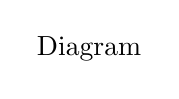
\begin{tikzpicture}
            \node at (0, 0) {Diagram};
        \end{tikzpicture}
    \end{center}

\begin{solution}
    \begin{center}
        \begin{tikzpicture}
            \pic at (0, 0) {frame=3cm};
        \end{tikzpicture}
    \end{center}

    \begin{align*}
        \intertext{From the conditions obtained in the previous problem, first we will check whether the mass \( m_2 \) goes up or down.}
        \intertext{Here, \( \dfrac{m_2}{m_1} = \eta > \sin \alpha + k \cos \alpha \), (substituting the values). Hence the mass \( m_2 \) will come down with an acceleration (say \( w \)). From the free body diagram of previous problem,}
        m_2 g - T &= m_2 w \tag{1}\\
        \intertext{and}
        T - m_1 g \sin \alpha - k m_1 g \cos \alpha &= m_1 w \tag{2}\\
        \intertext{Adding Eqs. (1) and (2), we get,}
        m_2 g - m_1 g \sin \alpha - k m_1 g \cos \alpha &= \left( m_1 + m_2 \right) w\\
        w &= \dfrac{\left( \dfrac{m_2}{m_1} - \sin \alpha - k \cos \alpha \right) g}{\left( 1 + \dfrac{m_2}{m_1} \right)} = \dfrac{\left( \eta - \sin \alpha - k \cos \alpha \right) g}{1 + \eta}
        \intertext{Substituting all the values,}
        w &= 0.048 \, g \approx 0.05 \, g\\
        \intertext{As \( m_2 \) moves down with acceleration of magnitude \( w = 0.05 \, g \) \( > 0 \), thus in vector form, acceleration of \( m_2 \) is given by}
        \vec{w}_2 &= \dfrac{\left( \eta - \sin \alpha - k \cos \alpha \right) g}{1 + \eta} = 0.05 \, g
    \end{align*}
\end{solution}
